\documentclass[a4paper,UKenglish,cleveref,autoref]{lipics-v2021}





\bibliographystyle{plainurl}

\title{Induced Disjoint Paths Without an Induced Minor}
\titlerunning{Induced Disjoint Paths Without an Induced Minor}



\author{Pierre Aboulker}{DIENS, \'Ecole normale sup\'erieure, CNRS, PSL University, Paris, France \and \url{https://www.di.ens.fr/~paboulker/} }{pierreaboulker@gmail.com}{}{}
\author{\'{E}douard Bonnet}{CNRS, ENS de Lyon, Université Claude Bernard Lyon 1, LIP UMR 5668, Lyon, France \and \url{http://perso.ens-lyon.fr/edouard.bonnet}}{edouard.bonnet@ens-lyon.fr}{https://orcid.org/0000-0002-1653-5822}{}
\author{Timothé Picavet}{LaBRI, Université de Bordeaux, France}{timothe.picavet@u-bordeaux.fr}{https://orcid.org/0000-0002-7129-0127}{}
\author{Nicolas Trotignon}{CNRS, ENS de Lyon, Université Claude Bernard Lyon 1, LIP UMR 5668, Lyon, France \and \url{http://perso.ens-lyon.fr/nicolas.trotignon}}{nicolas.trotignon@ens-lyon.fr}{}{}



\authorrunning{P. Aboulker, \'E. Bonnet, T. Picavet, N. Trotignon}

\Copyright{Pierre Aboulker, Édouard Bonnet, Timothé Picavet, Nicolas Trotignon}





\category{}

\relatedversion{}

\supplement{}



\acknowledgements{We thank Théo Pierron and Jean-Florent Raymond with whom this project started. We also thank Tuukka Korhonen, Daniel Lokshtanov, and Martin Milanič for some discussions, and in particular for asking about the flow problem (as opposed to the linkage one).}

\nolinenumbers 

\hideLIPIcs  

\EventEditors{John Q. Open and Joan R. Access}
\EventNoEds{2}
\EventLongTitle{42nd Conference on Very Important Topics (CVIT 2016)}
\EventShortTitle{CVIT 2016}
\EventAcronym{CVIT}
\EventYear{2016}
\EventDate{December 24--27, 2016}
\EventLocation{Little Whinging, United Kingdom}
\EventLogo{}
\SeriesVolume{42}
\ArticleNo{23}



\usepackage[utf8]{inputenc}  

\usepackage[T1]{fontenc}
\usepackage{lmodern}

\usepackage{amsmath}  
\usepackage{amssymb}
\usepackage{amsthm}
\usepackage{bbm}
\usepackage{accents}
\usepackage{complexity}

\usepackage{booktabs}
\usepackage{paralist}
\usepackage{fixmath}



\makeatletter
\newtheorem*{rep@theorem}{\rep@title}
\newcommand{\newreptheorem}[2]{\newenvironment{rep#1}[1]{\def\rep@title{#2 \ref{##1}}\begin{rep@theorem}}{\end{rep@theorem}}}
\makeatother

\newreptheorem{theorem}{Theorem}
\newreptheorem{lemma}{Lemma}
\newreptheorem{corollary}{Corollary}

\usepackage{pgfplots}
\usepackage{xspace}
\usepackage{tikz}
\usepackage{tikz-3dplot}

\usepackage[ruled,vlined,linesnumbered]{algorithm2e}

\usetikzlibrary{fit}
\usetikzlibrary{arrows}
\usetikzlibrary{patterns}
\usetikzlibrary{calc}
\usetikzlibrary{shapes}
\usetikzlibrary{positioning}
\usetikzlibrary{math}
\usetikzlibrary{shapes.symbols, shapes.geometric}
\usetikzlibrary{decorations.pathreplacing,calligraphy}
\usetikzlibrary{decorations.pathmorphing, backgrounds}
\usepackage[scr=boondox,scrscaled=1.05]{mathalfa}

\newcommand{\mis}{\textsc{Max Independent Set}\xspace}
\newcommand{\smis}{\textsc{MIS}\xspace}
\newcommand{\vc}{\textsc{Vertex Cover}\xspace}
\newcommand{\vcp}{\mathsf{vc}\xspace}
\newcommand{\wei}{\mathfrak{w}}

\renewcommand{\geq}{\geqslant}
\renewcommand{\leq}{\leqslant}
\renewcommand{\preceq}{\preccurlyeq}
\renewcommand{\succeq}{\succcurlyeq}
\renewcommand{\le}{\leq}
\renewcommand{\ge}{\geq}

\newcommand{\defparproblem}[4]{
 \vspace{1mm}
\noindent\fbox{
 \begin{minipage}{0.96\textwidth}
 \begin{tabular*}{\textwidth}{@{\extracolsep{\fill}}lr} #1 & {\bf{Parameter:}} #3 \\ \end{tabular*}
 {\bf{Input:}} #2 \\
 {\bf{Question:}} #4
 \end{minipage}
 }
 \vspace{1mm}
}

\newcommand{\arxiv}[1]{\href{http://arxiv.org/abs/#1}{arXiv:#1}}

\newcommand{\card}[1]{|{#1}|}

\DeclareMathOperator*{\bigland}{\bigwedge}
\DeclareMathOperator*{\biglor}{\bigvee}

\newtheorem{question}{Question}

\newenvironment{proofofclaim}{\noindent \textsc{Proof of the Claim:}}{\unskip\nobreak\hfill$\Diamond$\medskip}
  
\newcommand\subd[1]{#1\text{-subd}}
\newcommand\tw{\text{tw}}
\newcommand\tww{\text{tww}}


\begin{document}

\maketitle

\begin{abstract}
  We exhibit a new obstacle to the nascent algorithmic theory for classes excluding an induced minor.
  We indeed show that on the class of string graphs---which avoids the 1-subdivision of, say, $K_5$ as an induced minor---\textsc{Induced 2-Disjoint Paths} is NP-complete.
  So, while \textsc{$k$-Disjoint Paths}, for a~fixed $k$, is polynomial-time solvable in general graphs, the absence of a~graph as an induced minor does not make its induced variant tractable, even for $k=2$.
  This answers a~question of Korhonen and Lokshtanov [SODA~'24], and complements a~polynomial-time algorithm for \textsc{Induced $k$-Disjoint Paths} in classes of bounded genus by Kobayashi and Kawarabayashi [SODA~'09].
  In addition to being string graphs, our produced hard instances are subgraphs of a~constant power of bounded-degree planar graphs, hence have bounded twin-width and bounded maximum degree.
  
  We also leverage our new result to show that there is a fixed subcubic graph $H$ such that deciding if an input graph contains $H$ as an induced subdivision is NP-complete.
  Until now, all the graphs $H$ for which such a~statement was known had a~vertex of degree at~least~4.
  This answers a~question by Chudnovsky, Seymour, and the fourth author [JCTB '13], and by Le [JGT '19].
  Finally we resolve another question of Korhonen and Lokshtanov by exhibiting a~subcubic graph $H$ without two adjacent degree-3 vertices and such that deciding if an input $n$-vertex graph contains $H$ as an induced minor is NP-complete, and unless the Exponential-Time Hypothesis fails, requires time $2^{\Omega(\sqrt n)}$.
  This complements an algorithm running in subexponential time $2^{\Tilde{O}(n^{2/3})}$ by these authors [SODA~'24] under the same technical condition.
  \end{abstract}

\section{Introduction}\label{sec:intro}

In \textsc{$k$-Disjoint Paths}, one is given a~graph $G$, together with $k$ pairs of vertices, often called \emph{terminals}, $(s_1,t_1), \ldots, (s_k,t_k)$, and has to decide if $G$ admits $k$ vertex-disjoint paths $P_1, \ldots, P_k$ such that for every $i \in \{1, \ldots, k\}$, the endpoints of $P_i$ are $s_i$ and $t_i$.
This problem is also called \textsc{$k$-Linkage} as the pairs to connect are prescribed.
In the ``flow variant'' of this problem, \textsc{Disjoint $S$--$T$ Paths}, the input consists of a~graph $G$ and two disjoint vertex subsets $S, T \subset V(G)$ with $|S|=|T|$, and the question is whether there are $|S|$ vertex-disjoint paths, each with one endpoint in $S$ and the other endpoint in $T$.
These problems are polynomial-time solvable in general graphs, respectively by the work of Robertson and Seymour~\cite{Robertson95} (for \textsc{$k$-Disjoint Paths}), and simply by Menger's theorem~\cite{Menger27} (for \textsc{Disjoint $S$--$T$ Paths}).

In this paper, we are interested in their induced variants \textsc{Induced $k$-Disjoint Paths} and \textsc{Induced Disjoint $S$--$T$ Paths}, where the paths are further requested to be mutually induced (i.e., no edge of the graph is incident to two of these paths).
These problems are NP-complete for $k=2$ and for $|S|=|T|=2$, respectively, in general graphs~\cite{Fellows89,bienstock:evenpair}.
Note that \textsc{Induced Disjoint $S$--$T$ Paths} with $|S|=|T|=k$ can be solved with $k!$ calls to \textsc{Induced $k$-Disjoint Paths}.
So when $k$ is constant, the former problem is in principle simpler than the latter.

Kawarabayashi and Kobayashi give a~linear-time algorithm for \textsc{Induced $k$-Disjoint Paths} (for any fixed $k$) in planar graphs~\cite{KawarabayashiK12}, and a~polynomial-time algorithm in classes of bounded genus~\cite{KobayashiK09}.
The latter result is lifted to the model checking of the FO+SDP logic (i.e., first-order with \emph{scattered} disjoint paths predicates, which can natively express the existence of a~constant number of induced disjoint paths between some specified pairs of terminals) in fixed-parameter tractable (FPT) time in classes of bounded genus~\cite{GolovachST23}.
It is believed that the tractability of \textsc{Induced $k$-Disjoint Paths} (and perhaps even of FO+SDP model checking) holds more generally in classes excluding a~fixed minor, and could be shown by combining the irrelevant-vertex techniques (developed for the planar and bounded-genus cases) with the graph structure theorem of Robertson and Seymour~\cite{Robertson03}. 
However, to our knowledge, this has not been proven yet (provided it indeed holds).

\textsc{Induced $k$-Disjoint Paths} is polynomial-time solvable on classes of bounded mim-width on which mim-width can be efficiently approximated~\cite{Jaffke20}, which includes for instance interval graphs and permutation graphs.
In claw-free graphs (i.e., graphs excluding $K_{1,3}$ as an induced subgraph), \textsc{Induced $k$-Disjoint Paths} is solvable in polynomial time for any fixed $k$~\cite{DBLP:journals/algorithmica/FialaKLP12}, and even in FPT time in parameter~$k$~\cite{DBLP:journals/siamdm/GolovachPL15}.
In graphs without asteroidal triple, this problem is polynomial-time solvable even if~$k$ is part of the input~\cite{GolovachPL22}.
Finally, in (theta, wheel)-free graphs, there is a~polynomial-time algorithm for~\textsc{Induced $k$-Disjoint Paths} \cite{RadovanovicTV21}, while its complexity in theta-free graphs is open.

To understand better the tractability frontier of \textsc{Induced $k$-Disjoint Paths}, Korhonen and Lokshtanov~\cite{KorhonenL23} ask if this problem is NP-hard in \mbox{$H$-induced}-minor-free graphs for some fixed $k$ and $H$.
We resolve this question already in the case when $k=2$ and $H$ is equal to the 1-subdivision of~$K_5$ (or of~$K_{3,3}$).
Indeed string graphs (i.e., intersection graphs of curves in the plane) exclude the 1-subdivision of any non-planar graph as an induced minor.  

\begin{theorem}\label{thm:hardness-I2DP}
  \textsc{Induced 2-Disjoint Paths} is NP-complete in string graphs that are subgraphs of a~constant power of bounded-degree planar graphs.
\end{theorem}

We actually show the stronger result that \textsc{Induced Disjoint $S$--$T$ Paths} with $|S|=|T|=2$ is NP-complete in this subclass of string graphs. 
Note that subgraphs of constant powers of bounded-degree planar graphs both have bounded twin-width~\cite{twin-width1,twin-width2} and bounded maximum degree.
Thus \cref{thm:hardness-I2DP} considerably limits the scope within which the existing polynomial algorithms could be extended.

The Exponential-Time Hypothesis (ETH for short), a~stronger assumption than \mbox{P $\neq$ NP} but still widely believed, asserts that there is a~real $\lambda>1$ such that $n$-variable \textsc{3-SAT} cannot be solved in time~$O(\lambda^n)$~\cite{Impagliazzo01}.
More quantitatively, \cref{thm:hardness-I2DP}, by providing a~linear reduction from a~variant of \textsc{Planar 3-SAT} (see~\cite{Lichtenstein82}), implies the following.
\begin{corollary}\label{cor:tww}
  \textsc{Induced Disjoint $S$--$T$ Paths} with $|S|=|T|=2$ is NP-complete in string graphs of bounded maximum degree and twin-width, and requires time $2^{\Omega(\sqrt n)}$ on $n$-vertex such graphs, unless the Exponential-Time Hypothesis fails.
\end{corollary}

Our result has some consequences for the detection of induced subdivisions, which we now turn our attention to.

\paragraph*{Detecting induced subdivisions and induced minors}

Let \textsc{$H$-Induced Subdivision Containment} (\textsc{$H$-ISC} for short) input a~graph~$G$ and ask whether $H$ is an induced subdivision of~$G$.
This problem has attracted some attention.
Chudnovsky and Seymour introduced the \textsc{Three-In-A-Tree} problem---whether there is an induced subtree containing three given vertices---and showed how to solve it in polynomial time via the so-called extended strip decompositions, in order to obtain a~polynomial algorithm for \textsc{$K_{2,3}$-ISC}~\cite{DBLP:journals/combinatorica/ChudnovskyS10}.
The first graphs $H$ for which \textsc{$H$-ISC} is NP-complete came from~\cite{LevequeLMT09} where several examples are given: notably the complete graph $K_5$ and some trees, among other graphs.
In the same paper, some other examples of tractable \textsc{$H$-ISC} were given, all relying on the polynomial-time algorithm for \textsc{Three-In-A-Tree}.
There are also some ad hoc algorithms for \textsc{$H$-ISC} when $H$ is the \emph{net} (i.e., the graph obtained by adding a pendant neighbor to each vertex of a~triangle)~\cite{DBLP:journals/jct/ChudnovskyST13}, when $H$ is $K_4$~\cite{DBLP:journals/jgt/Le19}, or when $H$ is the disjoint union of a~fixed number of triangles~\cite{DBLP:journals/jctb/NguyenSS24}.

Despite this line of work, no subcubic graph $H$ was known to make \textsc{$H$-ISC} NP-hard.
Actually, Chudnovsky, Seymour, and the fourth author~\cite{DBLP:journals/jct/ChudnovskyST13} and Le~\cite{DBLP:journals/jgt/Le19} asked whether there is a~polynomial-time algorithm for \textsc{$H$-ISC} for any subcubic graph~$H$.
As a~consequence of~\cref{thm:hardness-I2DP}, we answer this question by the negative by exhibiting a~subcubic graph $H$ (the graph of~\cref{fig:H}) for which \textsc{$H$-ISC} is NP-hard.

\begin{figure}[h!]
  \centering
  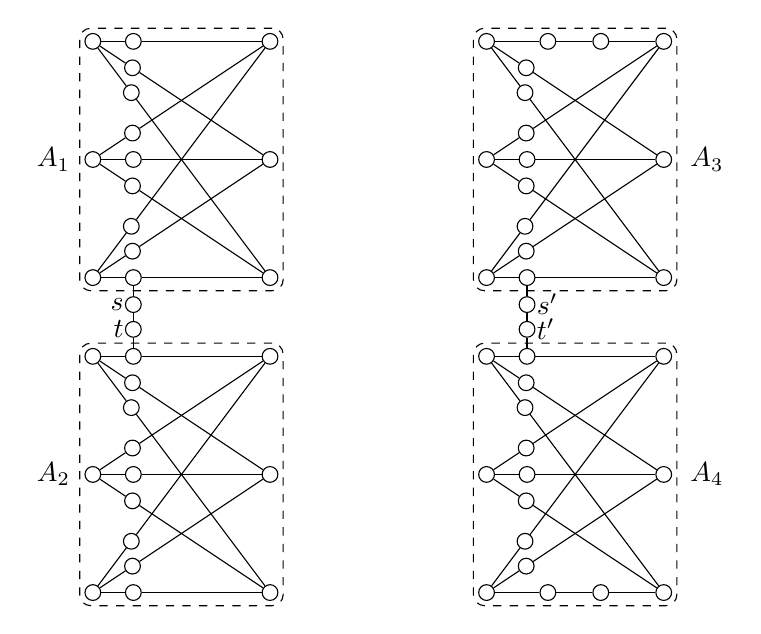
\begin{tikzpicture}[vertex/.style={draw,circle,inner sep=0.05cm, minimum width=0.2cm}]
    \def\s{1.5}

    \foreach \x/\y/\l in {0/0/1, 0/4/2}{
    \begin{scope}[xshift=\x cm, yshift = \y cm] 
      
    \foreach \i in {1,2,3}{
      \node[vertex] (u\l\i) at (0,\i * \s) {} ;
      \node[vertex] (v\l\i) at (1.5 * \s,\i * \s) {} ;
    }
    \node[draw,thin,dashed,rounded corners, inner sep=0.06cm, fit=(u\l1) (v\l3)] {} ;
    
    \foreach \i in {1,2,3}{
      \foreach \j in {1,2,3}{
        \path (u\l\i) to node[vertex, pos=0.2] (w\l\i\j) {} (v\l\j) ;
        \draw (u\l\i) -- (w\l\i\j) -- (v\l\j) ;
      }
    }

    \end{scope}
    }

    \foreach \x/\y/\l in {5/0/3, 5/4/4}{
    \begin{scope}[xshift=\x cm, yshift = \y cm] 
      
    \foreach \i in {1,2,3}{
      \node[vertex] (u\l\i) at (0,\i * \s) {} ;
      \node[vertex] (v\l\i) at (1.5 * \s,\i * \s) {} ;
    }
    \node[draw,thin,dashed,rounded corners, inner sep=0.06cm, fit=(u\l1) (v\l3)] {} ;
    
    \foreach \i/\j in {1/2,1/3,2/1,2/2,2/3,3/1,3/2}{
      \path (u\l\i) to node[vertex, pos=0.2] (w\l\i\j) {} (v\l\j) ;
      \draw (u\l\i) -- (w\l\i\j) -- (v\l\j) ;
    }

    \end{scope}
    }
    \path (u43) to node[vertex, pos=0.33] (w433) {} (v43) ;
    \path (u43) to node[vertex, pos=0.66] (w433b) {} (v43) ;
    \draw (u43) -- (w433) -- (w433b) -- (v43) ;

    \path (u41) to node[vertex, pos=0.2] (w411) {} (v41) ;
    \draw (u41) -- (w411) -- (v41) ;

    \path (u31) to node[vertex, pos=0.33] (w311) {} (v31) ;
    \path (u31) to node[vertex, pos=0.66] (w311b) {} (v31) ;
    \draw (u31) -- (w311) -- (w311b) -- (v31) ;

    \path (u33) to node[vertex, pos=0.2] (w333) {} (v33) ;
    \draw (u33) -- (w333) -- (v33) ;

\path (w133) to node[vertex, pos=0.3] (t) {} (w211) ;
    \path (w133) to node[vertex, pos=0.7] (s) {} (w211) ;
    \draw (w133) -- (t) -- (s)-- (w211) ;

    \path (w333) to node[vertex, pos=0.3] (tp) {} (w411) ;
    \path (w333) to node[vertex, pos=0.7] (sp) {} (w411) ;
    \draw (w333) -- (tp) -- (sp) -- (w411) ;

    \node[left] at (s) {$s$};
    \node[left] at (t) {$t$};
    \node[right] at (sp) {$s'$};
    \node[right] at (tp) {$t'$};

    \node at (-0.5,7) {$A_1$} ;
    \node at (-0.5,2 * \s) {$A_2$} ;

     \node at (7.8,7) {$A_3$} ;
    \node at (7.8,2 * \s) {$A_4$} ;
    
  \end{tikzpicture}
  \caption{The subcubic graph~$H$.
   Both $H[A_1]$ and $H[A_2]$ are the 1-subdivision of $K_{3,3}$.
  Both $H[A_3]$ and $H[A_4]$ are obtained from $K_{3,3}$ by subdividing every edge once but one edge that is subdivided twice.
  The vertices of $H$ which are not in $\bigcup_{i \in [4]} A_i$ are labeled $s, t, s', t'$.
  In total $H$ has 66 vertices.}
  \label{fig:H}
\end{figure}

\begin{theorem}\label{thm:hardness-subcubic-subd}
  \textsc{$H$-Induced Subdivision Containment} is NP-complete for the subcubic graph $H$ of~\cref{fig:H}.
\end{theorem}

\Cref{thm:hardness-subcubic-subd} holds within subgraphs of a~constant power of bounded-degree planar graphs that are string graphs plus a~constant number of (bounded-degree) apices, which are graphs of bounded twin-width~\cite{twin-width1,twin-width2} excluding a~fixed induced minor.
In other words, \cref{thm:hardness-subcubic-subd} holds in the graphs for which~\cref{thm:hardness-I2DP} holds augmented by a~constant number of vertices of bounded degree.

\medskip

\Cref{thm:hardness-I2DP} also has consequences for the detection of induced minors, topic that we now briefly survey.  
Let \textsc{$H$-Induced Minor Containment} (\textsc{$H$-IMC} for short) input a~graph~$G$ and ask whether $H$ is an induced minor of~$G$.
It was first shown by Fellows et al.~\cite{Fellows95} that \textsc{$H$-IMC} can be NP-hard for a~fixed graph~$H$ (unlike the minor containment).
The latter graph $H$ was not planar, which prompted the authors to ask if there is a~planar graph~$H$ for which \textsc{$H$-IMC} is NP-hard, and whether \textsc{$H$-IMC} is always polynomial-time solvable when $H$ is a~tree.
Recently, Korhonen and Lokshtanov~\cite{KorhonenL23} answered both questions by showing that \textsc{$H$-IMC} is NP-hard for some fixed tree~$H$ (whose number of vertices is not explicit, and estimated to be larger than $2^{300}$ in~\cite{Dallard25}).
Dallard et al.~\cite{Dallard24} show that \textsc{$K_{2,3}$-IMC} can be solved in polynomial time.
Finding the disjoint union of a~constant number of triangles as an induced minor or as an induced subdivision is all the same, so for any natural~$t$, \textsc{$tK_3$-IMC} is also in P~\cite{DBLP:journals/jctb/NguyenSS24}.
For a~more complete survey on the complexity of \textsc{$H$-IMC}, we refer the reader to the introduction of~\cite{Dallard25}; the paper provides some polynomial-time algorithms for three infinite families of graphs~$H$, and notes that \textsc{$H$-IMC} is in P for every graph $H$ on at~most 5 vertices, except for three remaining open cases.

As a~similar consequence to \Cref{cor:tww}, we show a~$2^{\Omega(\sqrt{n})}$ lower bound for \textsc{$H$-IMC} on $n$-vertex graphs, under the ETH.
This can be put in perspective with a~$2^{\tilde{O}(n^{2/3})}$-time algorithm for \textsc{$H$-IMC} when every edge of~$H$ is incident to a~vertex of degree at~most~2~\cite{KorhonenL23}.
The authors ask if the mere NP-hardness of \textsc{$H$-IMC} can be shown for some graph $H$ with this property. 
Actually by subdividing eight edges in the graph of~\cref{fig:H}, we obtain a~graph $H'$ satisfying the property, and for which we can show the same lower bound.

\begin{theorem}\label{thm:hardness-subcubic-ind-minor}
  There is a~subcubic graph $H'$ such that every edge of $H'$ is incident to a~vertex of~degree~2, and \textsc{$H'$-Induced Minor Containment} is NP-complete, and requires time $2^{\Omega(\sqrt n)}$ on $n$-vertex graphs, unless the ETH fails.
\end{theorem}

We observe that it is not too difficult to show~\cref{thm:hardness-subcubic-subd,thm:hardness-subcubic-ind-minor} with \emph{connected} graphs $H$ and $H'$ (having the extra properties of their respective statement).
As this complicates a~bit their proofs without being a~significantly stronger result, we opted against doing it explicitly.

\paragraph*{Open questions}

We suggest the following open questions, which come more or less directly from our work and the literature.
In light of the surveyed polynomial algorithms applying more generally to \textsc{Induced $k$-Disjoint Paths} and the hardness proofs applying more generally to \textsc{Induced Disjoint $S$--$T$ Paths} with $|S|=|T|=k$, we wonder if there is a hereditary graph class in which \textsc{Induced $k$-Disjoint Paths} is NP-complete but \textsc{Induced Disjoint $S$--$T$ Paths} with $|S|=|T|=k$ is polynomial-time solvable; the case $k=2$ is of particular interest.  

The string graphs that our proof of~\cref{thm:hardness-I2DP} produces do not seem to be 1-string graphs (i.e., realizable with strings every pair of which intersects at~most~once).
We leave open the complexity of \textsc{Induced $k$-Disjoint Paths} in 1-string graphs, and also in segment intersection graphs (a~further restriction to 1-string graphs).

A~natural conjecture stems from our paper and existing algorithms, under P $\neq$ NP.
\begin{conjecture}\label{conj:subcubic-subd-planar}
 For any subcubic graph $H$, \textsc{$H$-ISC} is in P if and only if $H$ is planar.
\end{conjecture}

\section{Preliminaries}

If $i$ is a~positive integer, we denote by $[i]$ the set of integers $\{1,2,\ldots,i\}$.

\subsection{Subgraphs, induced subgraphs, neighborhoods, and some graphs}\label{sec:graph-def}

We denote by $V(G)$ and $E(G)$ the set of vertices and edges of a graph $G$, respectively.
A~graph $H$ is a~\emph{subgraph} of a~graph $G$ if $H$ can be obtained from $G$ by vertex and edge deletions.
Graph~$H$ is an~\emph{induced subgraph} of $G$ if $H$ is obtained from $G$ by vertex deletions only.
A~graph $G$ is \emph{$H$-free} if $G$ does not contain $H$ as an induced subgraph.
For $S \subseteq V(G)$, the \emph{subgraph of $G$ induced by $S$}, denoted $G[S]$, is obtained by removing from $G$ all the vertices that are not in $S$ (together with their incident edges).
Then $G-S$ is a short-hand for $G[V(G)\setminus S]$.
A collection of paths $P_1, \ldots, P_h$ in a~graph $G$ is said \emph{mutually induced} if $G[\bigcup_{i \in [h]} V(P_i)]$ is exactly the disjoint union of paths $P_1, \ldots, P_h$.

A~set $X \subseteq V(G)$ is connected (in $G$) if $G[X]$ has a~single connected component.
A~vertex whose removal increases the number of connected components is called a~\emph{cutvertex}.
Similarly, a~\emph{bridge} is an edge whose removal increases the number of connected components.
We denote by $G^r$ the \emph{$r$-th power of $G$}, that is, the graph with vertex set $V(G)$ and an edge between any two vertices at (shortest-path) distance at~most~$r$ in~$G$.
A~\emph{constant power} of~$G$ is $G^r$ for some constant~$r$. 

A~\emph{subdivision} of a~graph $G$ is any graph obtained from $G$ by replacing each edge of~$G$ by a~path of at~least~one edge.
In a~subdivision of~$G$ the vertices of~$G$ are called \emph{branching vertices}, and the created vertices are called \emph{subdivision vertices}.
The \emph{$s$-subdivision} of $G$ is the graph obtained from $G$ by replacing each edge of~$G$ by a~path of $s+1$ edges.
 
We denote by $N_G(v)$ and $N_G[v]$, the open, respectively closed, neighborhood of $v$ in $G$.
For $S \subseteq V(G)$, we set $N_G(S) := (\bigcup_{v \in S}N_G(v)) \setminus S$ and $N_G[S] := N_G(S) \cup S$.
The \emph{degree} $d_G(v)$ of a~vertex $v \in V(G)$ is the cardinality of $N_G(v)$, and the \emph{maximum degree} of $G$ is defined as $\max_{v \in V(G)} d_G(v)$.
A~\emph{subcubic graph} is a~graph of maximum degree at most~3.

The \emph{$t$-clique}, denoted by \emph{$K_t$}, is obtained by making adjacent every pair of two distinct vertices among $t$ vertices, and the \emph{biclique $K_{t,t}$} with bipartition $(A,B)$ such that $|A|=|B|=t$ is obtained by making every vertex of~$A$ adjacent to every vertex of~$B$.  
A~\emph{theta} is any subdivision of $K_{2,3}$.
A~\emph{wheel} is any graph obtained by adding to a~cycle of length at~least~4, a~vertex with at~least three neighbors on the cycle.

A~\emph{string graph} is the intersection graph of some collection of (non-self-intersecting) curves in the plane (usually called strings), or equivalently the intersection graph of a~collection of connected sets of some planar graph.
The collection of strings is called \emph{string representation}.
We may see the string representation as a~planar diagram with one vertex at each string endpoint and at each intersection of two strings.
For instance, any string representation defines an infinite face (the infinite face of this planar diagram).

It is known (and easy to see) that the 1-subdivision of any non-planar graph is not a~string graph~\cite{Sinden66}.

\subsection{Induced subdivisions and induced minors}\label{sec:induced-subd-min}

A~graph $H$ is an induced subdivision of a~graph~$G$ if a~subdivision of~$H$ is isomorphic to an induced subgraph of~$G$.
An \emph{induced subdivision model} of $H$ in $G$ is given by an injective map $\phi: V(H) \to V(G)$ and a~collection of paths $(P_e)_{e \in E(H)}$ in $G$ such that for every $uv \in E(H)$, $P_{uv}$ is a~$\phi(u)$--$\phi(v)$ path, and $G[\bigcup_{e \in E(H)} V(P_e)]$ has no more edges than the paths $(P_e)_{e \in E(H)}$ themselves. 

An~\emph{induced minor model} of $H$ in~$G$ is a~collection $\mathcal M := \{X_1, \ldots, X_{|V(H)|}\}$ of pairwise-disjoint connected subsets of $V(G)$, called \emph{branch sets}, together with a~bijective map $\phi: V(H) \to \mathcal M$ such that $uv \in E(H)$ if and only if there is at~least one edge in $G$ between $\phi(u)$ and $\phi(v)$.
In which case, we may say that the branch sets $\phi(u)$ and $\phi(v)$ are \emph{adjacent}.
We then say that $H$ is an \emph{induced minor} of $G$ (or otherwise that $G$ is $H$-induced-minor-free).
Or equivalently, $H$ can be obtained from $G$ after a~series of~vertex deletions and edge contractions.

An induced minor model $(\{X_1, \ldots, X_h\}, \phi)$ of an $h$-vertex graph $H$ is \emph{minimal} if for every $X'_1 \subseteq X_1, \ldots, X'_h \subseteq X_h$, the fact that $(\{X'_1, \ldots, X'_h\}, \phi')$ is an induced minor model of~$H$ with $\phi'(u) = X'_i \Leftrightarrow \phi(u) = X_i$ for every $u \in V(H)$, implies that for every $i \in [h]$, $X'_i = X_i$.

With the second given definition of string graphs (see end of~\cref{sec:graph-def}), it is easy to see that the class of string graphs is closed under taking induced minors.
Thus no string graph admits the 1-subdivision of a~non-planar graph as an induced minor. 

\subsection{Useful facts on twin-width}

As we only mention twin-width in side remarks, we refrain from giving a~definition.
We list the theorems useful in~\cref{sec:i2dp}.
This can be read in a~black-box fashion.

It was first proven in~\cite{twin-width1} that the class of planar graphs has bounded twin-width.
The current best upper bound is~8~\cite{HlinenyJ23}.

\begin{theorem}[Theorem 6.3 in \cite{twin-width1}, \cite{HlinenyJ23}]\label{thm:planar-tww}
  Planar graphs have bounded twin-width, more precisely upper bounded by~8.
\end{theorem}

The constant powers of bounded twin-width graphs have bounded twin-width, as a~special case of so-called first-order transductions.

\begin{theorem}[Theorem 8.1 in \cite{twin-width1}]\label{thm:power-tww}
  There is a~function $f$ such that for any graph $G$ of twin-width~$d$ and for any positive integer~$r$, $G^r$ has twin-width at~most~$f(d,r)$.
\end{theorem}

Among weakly sparse classes (excluding a~$K_{t,t}$ as a~subgraph), the subgraph closure of any class of bounded twin-width has bounded twin-width.  

\begin{theorem}[\cite{twin-width2}]\label{thm:ws-subgraph-closure}
  There is a~function $g$ such that for any graph $G$ of twin-width~$d$ excluding~$K_{t,t}$ as a~subgraph (or in particular, of maximum degree at~most~$t-1$), then any subgraph of~$G$ has twin-width at~most~$g(d,t)$. 
\end{theorem}

\section{Hardness of \textsc{Induced 2-Disjoint Paths} in string graphs}\label{sec:i2dp}

In this section, we show that \textsc{Induced 2-Disjoint Paths} is NP-complete in (a~proper subclass of) string graphs.

\begin{reptheorem}{thm:hardness-I2DP}
  \textsc{Induced 2-Disjoint Paths} is NP-complete in string graphs that are subgraphs of a~constant power of bounded-degree planar graphs.
\end{reptheorem}

\begin{proof}\textcolor{red}{TOPROVE 0}\end{proof}

We then derive the following.

\begin{repcorollary}{cor:tww}
  \textsc{Induced Disjoint $S$--$T$ Paths} with $|S|=|T|=2$ is NP-complete in string graphs of bounded maximum degree and twin-width, and requires time $2^{\Omega(\sqrt n)}$ on $n$-vertex such graphs, unless the Exponential-Time Hypothesis fails.
\end{repcorollary}
\begin{proof}\textcolor{red}{TOPROVE 1}\end{proof}

\section{Hardness of detecting a subcubic graph as an induced subdivision}\label{sec:isc-imc}

As a~consequence of the previous section, we can prove~\cref{thm:hardness-subcubic-subd}, which we recall.

\begin{reptheorem}{thm:hardness-subcubic-subd}
  \textsc{$H$-Induced Subdivision Containment} is NP-complete for the subcubic graph $H$ of~\cref{fig:H}.
\end{reptheorem}

\begin{proof}\textcolor{red}{TOPROVE 2}\end{proof}

The previous reduction also works for \textsc{$H$-Induced Minor Containment}.
However, the proof is slightly more involved.
We tune $H$ a~little bit such that it is still subcubic but has no two adjacent vertices of degree~3 (so that the forthcoming result answers a~question of Korhonen and Lokshtanov).
We call the resulting graph~$H'$; see~\cref{fig:Hp}.
\begin{figure}[h!]
  \centering
  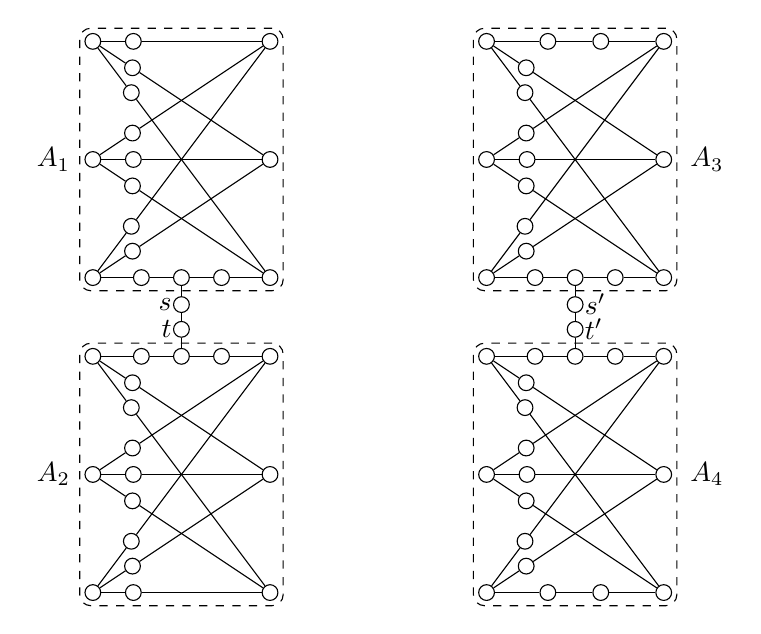
\begin{tikzpicture}[vertex/.style={draw,circle,inner sep=0.05cm, minimum width=0.2cm}]
    \def\s{1.5}

    \foreach \x/\y/\l in {0/0/1, 0/4/2}{
    \begin{scope}[xshift=\x cm, yshift = \y cm] 
      
    \foreach \i in {1,2,3}{
      \node[vertex] (u\l\i) at (0,\i * \s) {} ;
      \node[vertex] (v\l\i) at (1.5 * \s,\i * \s) {} ;
    }
    \node[draw,thin,dashed,rounded corners, inner sep=0.06cm, fit=(u\l1) (v\l3)] {} ;
    
    \foreach \i/\j in {1/2,1/3,2/1,2/2,2/3,3/1,3/2}{
      \path (u\l\i) to node[vertex, pos=0.2] (w\l\i\j) {} (v\l\j) ;
      \draw (u\l\i) -- (w\l\i\j) -- (v\l\j) ;
    }

    \end{scope}
    }

    \foreach \x/\y/\l in {5/0/3, 5/4/4}{
    \begin{scope}[xshift=\x cm, yshift = \y cm] 
      
    \foreach \i in {1,2,3}{
      \node[vertex] (u\l\i) at (0,\i * \s) {} ;
      \node[vertex] (v\l\i) at (1.5 * \s,\i * \s) {} ;
    }
    \node[draw,thin,dashed,rounded corners, inner sep=0.06cm, fit=(u\l1) (v\l3)] {} ;
    
    \foreach \i/\j in {1/2,1/3,2/1,2/2,2/3,3/1,3/2}{
      \path (u\l\i) to node[vertex, pos=0.2] (w\l\i\j) {} (v\l\j) ;
      \draw (u\l\i) -- (w\l\i\j) -- (v\l\j) ;
    }

    \end{scope}
    }
\path (u43) to node[vertex, pos=0.33] (w433) {} (v43) ;
    \path (u43) to node[vertex, pos=0.66] (w433b) {} (v43) ;
    \draw (u43) -- (w433) -- (w433b) -- (v43) ;

    \path (u41) to node[vertex, pos=0.25] (w411l) {} (v41) ;
    \path (u41) to node[vertex, pos=0.75] (w411r) {} (v41) ;
    \path (u41) to node[vertex, pos=0.5] (w411) {} (v41) ;
    \draw (u41) -- (w411l) -- (w411) -- (w411r)  -- (v41) ;

    \path (u31) to node[vertex, pos=0.33] (w311) {} (v31) ;
    \path (u31) to node[vertex, pos=0.66] (w311b) {} (v31) ;
    \draw (u31) -- (w311) -- (w311b) -- (v31) ;

    \path (u33) to node[vertex, pos=0.25] (w333l) {} (v33) ;
    \path (u33) to node[vertex, pos=0.75] (w333r) {} (v33) ;
    \path (u33) to node[vertex, pos=0.5] (w333) {} (v33) ;
    \draw (u33) -- (w333l) -- (w333) -- (w333r) -- (v33) ;

    \path (u13) to node[vertex, pos=0.25] (w133l) {} (v13) ;
    \path (u13) to node[vertex, pos=0.5] (w133) {} (v13) ;
    \path (u13) to node[vertex, pos=0.75] (w133r) {} (v13) ;
    \draw (u13) -- (w133l) -- (w133) -- (w133r) -- (v13) ;
    
    \path (u21) to node[vertex, pos=0.25] (w211l) {} (v21) ;
    \path (u21) to node[vertex, pos=0.5] (w211) {} (v21) ;
    \path (u21) to node[vertex, pos=0.75] (w211r) {} (v21) ;
    \draw (u21) -- (w211l) -- (w211) -- (w211r) -- (v21) ;

    \path (u11) to node[vertex, pos=0.2] (w111) {} (v11) ;
    \draw (u11) -- (w111) -- (v11) ;

    \path (u23) to node[vertex, pos=0.2] (w233) {} (v23) ;
    \draw (u23) -- (w233) -- (v23) ;



\path (w133) to node[vertex, pos=0.3] (t) {} (w211) ;
    \path (w133) to node[vertex, pos=0.7] (s) {} (w211) ;
    \draw (w133) -- (t) -- (s)-- (w211) ;

    \path (w333) to node[vertex, pos=0.3] (tp) {} (w411) ;
    \path (w333) to node[vertex, pos=0.7] (sp) {} (w411) ;
    \draw (w333) -- (tp) -- (sp) -- (w411) ;

    \node[left] at (s) {$s$};
    \node[left] at (t) {$t$};
    \node[right] at (sp) {$s'$};
    \node[right] at (tp) {$t'$};


    \node at (-0.5,7) {$A_1$} ;
    \node at (-0.5,2 * \s) {$A_2$} ;

    \node at (7.8,7) {$A_3$} ;
    \node at (7.8,2 * \s) {$A_4$} ;
    
  \end{tikzpicture}
  \caption{
  The graph $H'$ obtained from $H$ of~\cref{fig:H} by subdividing in each $A_i$ the two edges incident to the vertex with a~neighbor in $\{s,t,s',t'\}$.
  In total $H'$ has 74 vertices. 
  }
  \label{fig:Hp}
\end{figure}

\begin{reptheorem}{thm:hardness-subcubic-ind-minor}
  There is a~subcubic graph $H'$ such that every edge of $H'$ is incident to a~vertex of~degree~2, and \textsc{$H'$-Induced Minor Containment} is NP-complete, and requires time $2^{\Omega(\sqrt n)}$ on $n$-vertex graphs, unless the ETH fails.
\end{reptheorem}

\begin{proof}\textcolor{red}{TOPROVE 3}\end{proof}

\begin{thebibliography}{10}

\bibitem{bienstock:evenpair}
Daniel Bienstock.
\newblock On the complexity of testing for odd holes and induced odd paths.
\newblock {\em Discret. Math.}, 90(1):85--92, 1991.
\newblock See also Corrigendum by B. Reed, {\it Discrete Mathematics},
  102:109--109, 1992.
\newblock \href {https://doi.org/10.1016/0012-365X(91)90098-M}
  {\path{doi:10.1016/0012-365X(91)90098-M}}.

\bibitem{twin-width2}
{\'{E}}douard Bonnet, Colin Geniet, Eun~Jung Kim, St{\'{e}}phan Thomass{\'{e}},
  and R{\'{e}}mi Watrigant.
\newblock {Twin-width II: small classes}.
\newblock {\em Combinatorial Theory}, 2(2), 2022.
\newblock URL: \url{https://escholarship.org/uc/item/9cs265b9}, \href
  {https://doi.org/http://dx.doi.org/10.5070/C62257876}
  {\path{doi:http://dx.doi.org/10.5070/C62257876}}.

\bibitem{twin-width1}
{\'{E}}douard Bonnet, Eun~Jung Kim, St{\'{e}}phan Thomass{\'{e}}, and
  R{\'{e}}mi Watrigant.
\newblock Twin-width {I:} tractable {FO} model checking.
\newblock {\em J. {ACM}}, 69(1):3:1--3:46, 2022.
\newblock \href {https://doi.org/10.1145/3486655} {\path{doi:10.1145/3486655}}.

\bibitem{DBLP:journals/combinatorica/ChudnovskyS10}
Maria Chudnovsky and Paul Seymour.
\newblock The three-in-a-tree problem.
\newblock {\em Combinatorica}, 30(4):387--417, 2010.
\newblock URL: \url{https://doi.org/10.1007/s00493-010-2334-4}, \href
  {https://doi.org/10.1007/S00493-010-2334-4}
  {\path{doi:10.1007/S00493-010-2334-4}}.

\bibitem{DBLP:journals/jct/ChudnovskyST13}
Maria Chudnovsky, Paul Seymour, and Nicolas Trotignon.
\newblock Detecting an induced net subdivision.
\newblock {\em Journal of Combinatorial Theory, series {B}}, 103(5):630--641,
  2013.
\newblock URL: \url{https://doi.org/10.1016/j.jctb.2013.07.005}, \href
  {https://doi.org/10.1016/J.JCTB.2013.07.005}
  {\path{doi:10.1016/J.JCTB.2013.07.005}}.

\bibitem{Dallard24}
Cl{\'{e}}ment Dallard, Ma{\"{e}}l Dumas, Claire Hilaire, Martin Milanic,
  Anthony Perez, and Nicolas Trotignon.
\newblock {Detecting $K_{2,3}$ as an Induced Minor}.
\newblock In Adele~Anna Rescigno and Ugo Vaccaro, editors, {\em Combinatorial
  Algorithms - 35th International Workshop, {IWOCA} 2024, Ischia, Italy, July
  1-3, 2024, Proceedings}, volume 14764 of {\em Lecture Notes in Computer
  Science}, pages 151--164. Springer, 2024.
\newblock \href {https://doi.org/10.1007/978-3-031-63021-7\_12}
  {\path{doi:10.1007/978-3-031-63021-7\_12}}.

\bibitem{Dallard25}
Clément Dallard, Maël Dumas, Claire Hilaire, and Anthony Perez.
\newblock Sufficient conditions for polynomial-time detection of induced
  minors, 2025.
\newblock URL: \url{https://arxiv.org/abs/2501.00161}, \href
  {http://arxiv.org/abs/2501.00161} {\path{arXiv:2501.00161}}.

\bibitem{Fellows89}
Michael~R. Fellows.
\newblock {The Robertson-Seymour theorems: A survey of applications}.
\newblock {\em Contemporary Mathematics}, 89:1--18, 1989.

\bibitem{Fellows95}
Michael~R. Fellows, Jan Kratochv{\'{\i}}l, Matthias Middendorf, and Frank
  Pfeiffer.
\newblock The complexity of induced minors and related problems.
\newblock {\em Algorithmica}, 13(3):266--282, 1995.
\newblock \href {https://doi.org/10.1007/BF01190507}
  {\path{doi:10.1007/BF01190507}}.

\bibitem{DBLP:journals/algorithmica/FialaKLP12}
Jir{\'{\i}} Fiala, Marcin Kaminski, Bernard Lidick{\'{y}}, and Dani{\"{e}}l
  Paulusma.
\newblock {The k-in-a-Path Problem for Claw-free Graphs}.
\newblock {\em Algorithmica}, 62(1-2):499--519, 2012.
\newblock URL: \url{https://doi.org/10.1007/s00453-010-9468-z}, \href
  {https://doi.org/10.1007/S00453-010-9468-Z}
  {\path{doi:10.1007/S00453-010-9468-Z}}.

\bibitem{DBLP:journals/siamdm/GolovachPL15}
Petr~A. Golovach, Dani{\"{e}}l Paulusma, and Erik~Jan van Leeuwen.
\newblock {Induced Disjoint Paths in Claw-Free Graphs}.
\newblock {\em {SIAM} J. Discret. Math.}, 29(1):348--375, 2015.
\newblock \href {https://doi.org/10.1137/140963200}
  {\path{doi:10.1137/140963200}}.

\bibitem{GolovachPL22}
Petr~A. Golovach, Dani{\"{e}}l Paulusma, and Erik~Jan van Leeuwen.
\newblock {Induced Disjoint Paths in AT-free graphs}.
\newblock {\em J. Comput. Syst. Sci.}, 124:170--191, 2022.
\newblock URL: \url{https://doi.org/10.1016/j.jcss.2021.10.003}, \href
  {https://doi.org/10.1016/J.JCSS.2021.10.003}
  {\path{doi:10.1016/J.JCSS.2021.10.003}}.

\bibitem{GolovachST23}
Petr~A. Golovach, Giannos Stamoulis, and Dimitrios~M. Thilikos.
\newblock Model-checking for first-order logic with disjoint paths predicates
  in proper minor-closed graph classes.
\newblock In Nikhil Bansal and Viswanath Nagarajan, editors, {\em Proceedings
  of the 2023 {ACM-SIAM} Symposium on Discrete Algorithms, {SODA} 2023,
  Florence, Italy, January 22-25, 2023}, pages 3684--3699. {SIAM}, 2023.
\newblock URL: \url{https://doi.org/10.1137/1.9781611977554.ch141}, \href
  {https://doi.org/10.1137/1.9781611977554.CH141}
  {\path{doi:10.1137/1.9781611977554.CH141}}.

\bibitem{HlinenyJ23}
Petr Hlinen{\'{y}} and Jan Jedelsk{\'{y}}.
\newblock Twin-width of planar graphs is at most 8, and at most 6 when
  bipartite planar.
\newblock In Kousha Etessami, Uriel Feige, and Gabriele Puppis, editors, {\em
  50th International Colloquium on Automata, Languages, and Programming,
  {ICALP} 2023, July 10-14, 2023, Paderborn, Germany}, volume 261 of {\em
  LIPIcs}, pages 75:1--75:18. Schloss Dagstuhl - Leibniz-Zentrum f{\"{u}}r
  Informatik, 2023.
\newblock URL: \url{https://doi.org/10.4230/LIPIcs.ICALP.2023.75}, \href
  {https://doi.org/10.4230/LIPICS.ICALP.2023.75}
  {\path{doi:10.4230/LIPICS.ICALP.2023.75}}.

\bibitem{Impagliazzo01}
Russell Impagliazzo and Ramamohan Paturi.
\newblock {On the Complexity of k-SAT}.
\newblock {\em J. Comput. Syst. Sci.}, 62(2):367--375, 2001.
\newblock \href {https://doi.org/10.1006/jcss.2000.1727}
  {\path{doi:10.1006/jcss.2000.1727}}.

\bibitem{sparsification}
Russell Impagliazzo, Ramamohan Paturi, and Francis Zane.
\newblock Which problems have strongly exponential complexity?
\newblock {\em J. Comput. Syst. Sci.}, 63(4):512--530, 2001.
\newblock \href {https://doi.org/10.1006/jcss.2001.1774}
  {\path{doi:10.1006/jcss.2001.1774}}.

\bibitem{Jaffke20}
Lars Jaffke, O{-}joung Kwon, and Jan~Arne Telle.
\newblock {Mim-Width I. Induced path problems}.
\newblock {\em Discret. Appl. Math.}, 278:153--168, 2020.
\newblock URL: \url{https://doi.org/10.1016/j.dam.2019.06.026}, \href
  {https://doi.org/10.1016/J.DAM.2019.06.026}
  {\path{doi:10.1016/J.DAM.2019.06.026}}.

\bibitem{KawarabayashiK12}
Ken{-}ichi Kawarabayashi and Yusuke Kobayashi.
\newblock A linear time algorithm for the induced disjoint paths problem in
  planar graphs.
\newblock {\em J. Comput. Syst. Sci.}, 78(2):670--680, 2012.
\newblock URL: \url{https://doi.org/10.1016/j.jcss.2011.10.004}, \href
  {https://doi.org/10.1016/J.JCSS.2011.10.004}
  {\path{doi:10.1016/J.JCSS.2011.10.004}}.

\bibitem{KobayashiK09}
Yusuke Kobayashi and Ken{-}ichi Kawarabayashi.
\newblock Algorithms for finding an induced cycle in planar graphs and bounded
  genus graphs.
\newblock In Claire Mathieu, editor, {\em Proceedings of the Twentieth Annual
  {ACM-SIAM} Symposium on Discrete Algorithms, {SODA} 2009, New York, NY, USA,
  January 4-6, 2009}, pages 1146--1155. {SIAM}, 2009.
\newblock \href {https://doi.org/10.1137/1.9781611973068.124}
  {\path{doi:10.1137/1.9781611973068.124}}.

\bibitem{KorhonenL23}
Tuukka Korhonen and Daniel Lokshtanov.
\newblock Induced-minor-free graphs: Separator theorem, subexponential
  algorithms, and improved hardness of recognition.
\newblock In David~P. Woodruff, editor, {\em Proceedings of the 2024 {ACM-SIAM}
  Symposium on Discrete Algorithms, {SODA} 2024, Alexandria, VA, USA, January
  7-10, 2024}, pages 5249--5275. {SIAM}, 2024.
\newblock \href {https://doi.org/10.1137/1.9781611977912.188}
  {\path{doi:10.1137/1.9781611977912.188}}.

\bibitem{DBLP:journals/jgt/Le19}
Ngoc{-}Khang Le.
\newblock Detecting an induced subdivision of {$K_4$}.
\newblock {\em Journal of Graph Theory}, 90(2):160--171, 2019.
\newblock URL: \url{https://doi.org/10.1002/jgt.22374}, \href
  {https://doi.org/10.1002/JGT.22374} {\path{doi:10.1002/JGT.22374}}.

\bibitem{LevequeLMT09}
Benjamin L{\'{e}}v{\^{e}}que, David~Y. Lin, Fr{\'{e}}d{\'{e}}ric Maffray, and
  Nicolas Trotignon.
\newblock Detecting induced subgraphs.
\newblock {\em Discret. Appl. Math.}, 157(17):3540--3551, 2009.
\newblock URL: \url{https://doi.org/10.1016/j.dam.2009.02.015}, \href
  {https://doi.org/10.1016/J.DAM.2009.02.015}
  {\path{doi:10.1016/J.DAM.2009.02.015}}.

\bibitem{Lichtenstein82}
David Lichtenstein.
\newblock Planar formulae and their uses.
\newblock {\em {SIAM} J. Comput.}, 11(2):329--343, 1982.
\newblock \href {https://doi.org/10.1137/0211025} {\path{doi:10.1137/0211025}}.

\bibitem{Menger27}
Karl Menger.
\newblock Zur allgemeinen kurventheorie.
\newblock {\em Fundamenta Mathematicae}, 10(1):96--115, 1927.

\bibitem{DBLP:journals/jctb/NguyenSS24}
Tung Nguyen, Alex~D. Scott, and Paul Seymour.
\newblock Induced paths in graphs without anticomplete cycles.
\newblock {\em J. Comb. Theory {B}}, 164:321--339, 2024.
\newblock URL: \url{https://doi.org/10.1016/j.jctb.2023.10.003}, \href
  {https://doi.org/10.1016/J.JCTB.2023.10.003}
  {\path{doi:10.1016/J.JCTB.2023.10.003}}.

\bibitem{RadovanovicTV21}
Marko Radovanovic, Nicolas Trotignon, and Kristina Vuskovic.
\newblock The (theta, wheel)-free graphs part {IV:} induced paths and cycles.
\newblock {\em J. Comb. Theory {B}}, 146:495--531, 2021.
\newblock URL: \url{https://doi.org/10.1016/j.jctb.2020.06.002}, \href
  {https://doi.org/10.1016/J.JCTB.2020.06.002}
  {\path{doi:10.1016/J.JCTB.2020.06.002}}.

\bibitem{Robertson95}
Neil Robertson and Paul Seymour.
\newblock {Graph Minors. XIII. The Disjoint Paths Problem}.
\newblock {\em Journal of Combinatorial Theory, Series B}, 63(1):65--110, 1995.
\newblock URL:
  \url{https://www.sciencedirect.com/science/article/pii/S0095895685710064},
  \href {https://doi.org/https://doi.org/10.1006/jctb.1995.1006}
  {\path{doi:https://doi.org/10.1006/jctb.1995.1006}}.

\bibitem{Robertson03}
Neil Robertson and Paul Seymour.
\newblock Graph minors. {XVI.} excluding a non-planar graph.
\newblock {\em J. Comb. Theory {B}}, 89(1):43--76, 2003.
\newblock \href {https://doi.org/10.1016/S0095-8956(03)00042-X}
  {\path{doi:10.1016/S0095-8956(03)00042-X}}.

\bibitem{Sinden66}
Frank~W. Sinden.
\newblock {Topology of thin film RC circuits}.
\newblock {\em Bell System Technical Journal}, 45(9):1639--1662, 1966.

\bibitem{Tippenhauer16}
Simon Tippenhauer and Wolfgang Muzler.
\newblock On planar {3-SAT} and its variants.
\newblock {\em Fachbereich Mathematik und Informatik der Freien Universitat
  Berlin}, 2016.

\end{thebibliography}

\end{document}
